\chapter{Sensores}
A fechadura utilizará apenas um tipo de sensor, o sensor de RFID que auxiliará
na autenticação.

O termo RFID é a sigla para identificação por radiofrequências (Radio Frequency
Identification), ou seja, é uma forma de por meio de ondas de rádio para identificação de
algo \cite{rouse2019}.

Um sistema RFID possui 3 componentes: uma antena, um transceptor e um
transponder. O transponder (etiqueta) é a identificação em si, cada transponder emite uma
frequência diferente. A antena tem a função de receber essa frequência do transponder e
repassá-la para o transceptor que converterá essa frequência para um sinal digital, que
será tratado por um outro componente, no nosso caso, o ATMEGA328p \cite{ciriaco2019}.

O transponder, também chamado de tag RFID, pode ser de dois tipos: ativo ou
passivo. Uma tag passiva é aquela que emite um sinal apenas como resposta ao sinal da
antena, já as tags ativas emitem seu próprio sinal, mas para isso precisam de uma bateria
interna.

\section{Módulo RFID RC522}

O módulo RC522 (Figura ~\ref{fig:rfid}) que utilizaremos é uma placa que contém a antena e
o transceptor. Ele se comunicará com o microcontrolador utilizando o protocolo ISP, por
isso precisa ser conectado conforme a tabela ~\ref{tab:rfidpinout} \cite{gbur2017}.

\FloatBarrier
\begin{figure}[!htbp]
	\centering
	\caption{Módulo RFID RC522}
	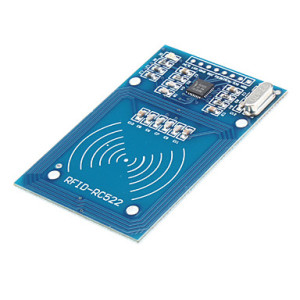
\includegraphics[scale=.3]{imagens/rfid}
	\\\textbf{Fonte:} \href{http://projectshopbd.com/product/rfid-rc522r15/}{Project Shop}
	\label{fig:rfid}
\end{figure}
\FloatBarrier

\FloatBarrier
\begin{table}[!htbp]
	\centering
	\caption{Conexões do RC522}
	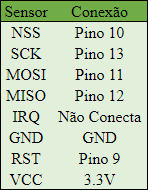
\includegraphics[scale=.5]{imagens/rfidpinout}
	\\ \vspace{0.2cm}
	\textbf{Fonte:} Elaborada pelos autores
	\label{tab:rfidpinout}
\end{table}
\FloatBarrier

\section{Teste do sensor}
O teste foi feito utilizando além do sensor, uma tela LCD,
que foi ligada ao circuito conforme a tabela ~\ref{tab:lcdpinout} \cite{componentes1012017}.
A tela exibiu o texto “Acesso liberado” quando o sensor leu
uma frequência aceita, caso a frequência lida tenha sido de
um cartão bloqueado a tela exibiu o texto “Bloqueado”,
e por fim, no caso de um cartão desconhecido, o texto
exibido foi “Acesso negado”.

\FloatBarrier
\begin{table}[!htbp]
	\centering
	\caption{Conexões do LCD}
	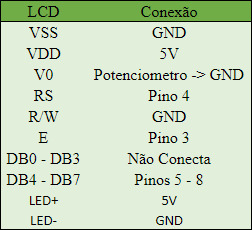
\includegraphics[scale=.5]{imagens/lcdpinout}
	\\ \vspace{0.2cm}
	\textbf{Fonte:} Elaborada pelos autores
	\label{tab:lcdpinout}
\end{table}
\FloatBarrier

O código utilizado para o teste do sensor está no Apêndice
~\ref{appendix:A}, e a figura ~\ref{fig:esquemasensores}
representa o esquema da montagem final para o teste.

\FloatBarrier
\begin{figure}[!htbp]
	\centering
	\caption{Esquema elétrico do teste dos sensores}
	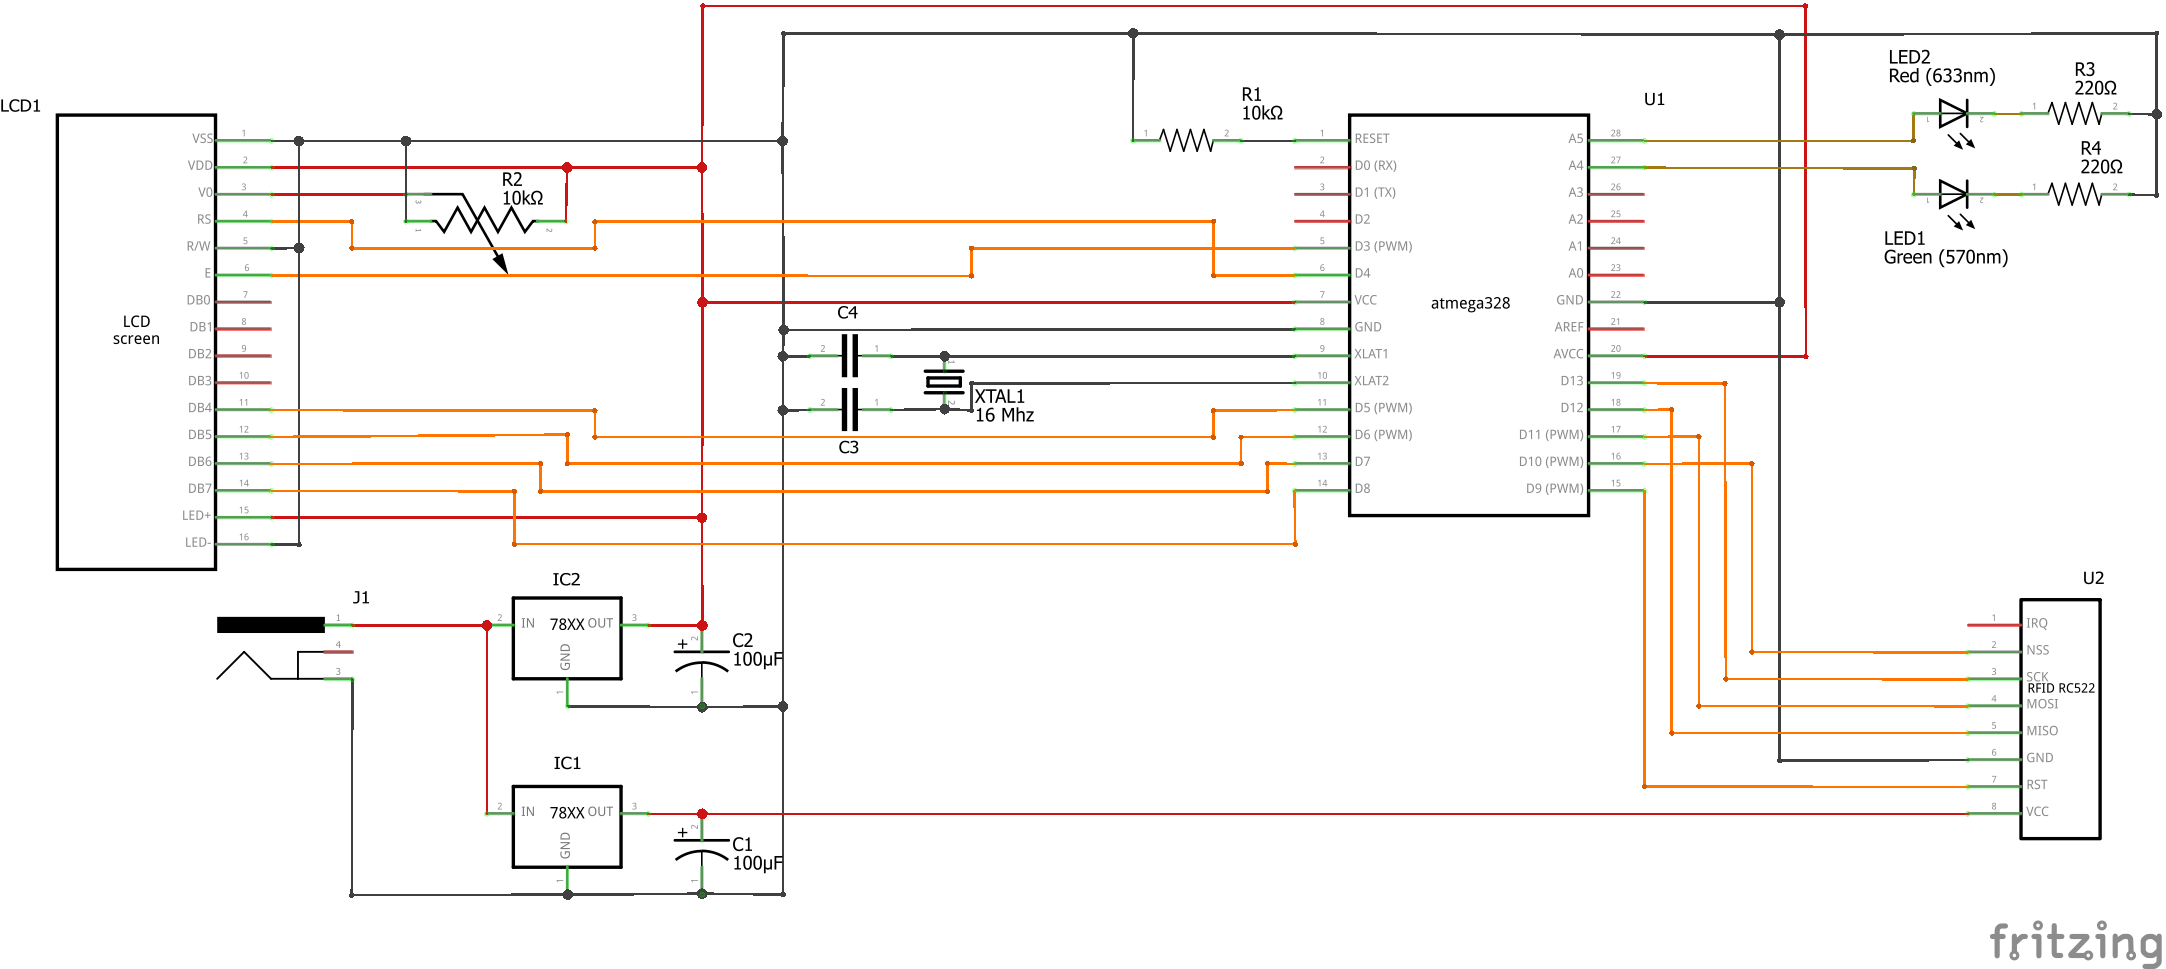
\includegraphics[scale=.7]{imagens/esquemasensores}
	\\\textbf{Fonte:} Elaborado pelos autores
	\label{fig:esquemasensores}
\end{figure}
\FloatBarrier
